%----------------------------------------------------------------------------------------
%	PACKAGES AND OTHER DOCUMENT CONFIGURATIONS
%----------------------------------------------------------------------------------------

\documentclass[11pt,fleqn]{book} % Default font size and left-justified equations

\usepackage[top=3cm,bottom=3cm,left=3.2cm,right=3.2cm,headsep=10pt,letterpaper]{geometry} % Page margins

\usepackage{xcolor} % Required for specifying colors by name
\definecolor{ocre}{RGB}{52,177,201} % Define the orange color used for highlighting throughout the book

% Font Settings
\usepackage{avant} % Use the Avantgarde font for headings
%\usepackage{times} % Use the Times font for headings
\usepackage{mathptmx} % Use the Adobe Times Roman as the default text font together with math symbols from the Sym­bol, Chancery and Com­puter Modern fonts
\usepackage{microtype} % Slightly tweak font spacing for aesthetics
\usepackage[utf8]{inputenc} % Required for including letters with accents
\usepackage[T1]{fontenc} % Use 8-bit encoding that has 256 glyphs

\usepackage{amsthm}
\usepackage{bbm}
\usepackage{amsmath}
\usepackage{xcolor}
\usepackage{bm}
\usepackage{tikz}
\usetikzlibrary{bayesnet}
\usepackage{subcaption}
\usepackage{float}
\usepackage{stackengine}
\usepackage{minted}
\usepackage{array}
\usepackage{multirow}
\usepackage{stmaryrd}
\usepackage{pgfplots}
\usepgfplotslibrary{fillbetween}
\usetikzlibrary{patterns}
\usetikzlibrary{shapes.geometric}
\usepackage[ruled,vlined]{algorithm2e}

\input{structure} % Insert the commands.tex file which contains the majority of the structure behind the template

%----------------------------------------------------------------------------------------
%	Definitions of new commands
%----------------------------------------------------------------------------------------

\pgfmathdeclarefunction{gauss}{3}{%
  \pgfmathparse{1/(#3*sqrt(2*pi))*exp(-((#1-#2)^2)/(2*#3^2))}%
}
\pgfmathdeclarefunction{sum_gauss}{5}{%
  \pgfmathparse{1/(3*#3*sqrt(2*pi))*exp(-((#1-#2)^2)/(2*#3^2)) + 2/(3*#5*sqrt(2*pi))*exp(-((#1-#4)^2)/(2*#5^2))}%
}
\newcommand{\fracpartial}[2]{\frac{\partial #1}{\partial  #2}}
\newcommand{\kl}[2]{D_{\mathrm{KL}} \left[ \left. \left. #1 \right|\right| #2 \right] }
\DeclareMathOperator*{\argmax}{arg\,max}
\DeclareMathOperator*{\argmin}{arg\,min}
\definecolor{blue-violet}{rgb}{0.54, 0.17, 0.89}
\definecolor{bluepigment}{rgb}{0.2, 0.2, 0.6}
\makeatletter
\newcommand*\bigcdot{\mathpalette\bigcdot@{.5}}
\newcommand*\bigcdot@[2]{\mathbin{\vcenter{\hbox{\scalebox{#2}{$\m@th#1\bullet$}}}}}
\makeatother
\def\delequal{\mathrel{\ensurestackMath{\stackon[1pt]{=}{\scriptstyle\Delta}}}}
\definecolor{Yellow}{RGB}{211, 176, 15}
\definecolor{Green}{rgb}{0.01, 0.75, 0.24}
\colorlet{Red}{red!50!black}
\colorlet{Blue}{blue!50!black}
\definecolor{Violet}{rgb}{0.56,0.14,0.56}
\newcommand{\indep}{\perp \! \! \! \perp}
\def\R{\mathbb{R}}

\begin{document}

%----------------------------------------------------------------------------------------
%	TITLE PAGE
%----------------------------------------------------------------------------------------

\begingroup
\thispagestyle{empty}
\AddToShipoutPicture*{\put(0,0){\includegraphics[scale=1.25]{TitlePageImage}}} % Image background
\centering
\vspace*{5cm}
\par\normalfont\fontsize{35}{35}\sffamily\selectfont
\textbf{Artificial Intelligence}\\
{\LARGE by Théophile Champion}\par % Book title
\vspace*{1cm}
{\Huge Research Notes}\par % Author name
\endgroup

%----------------------------------------------------------------------------------------
%	COPYRIGHT PAGE
%----------------------------------------------------------------------------------------

\newpage
~\vfill
\thispagestyle{empty}

%\noindent Copyright \copyright\ 2014 Andrea Hidalgo\\ % Copyright notice

\noindent \textsc{Doctor of Philosophy, University of Kent}\\

\noindent \textsc{github.com/ChampiB}\\ % URL

\noindent This research was done under the supervision of Pr. Howard Bowman and Dr. Marek Grze\'s with the financial support of the University of Kent within a total of 3 years, from September 2019 to September 2022.\\

\noindent \textit{First release, August 2022} % Printing/edition date

%----------------------------------------------------------------------------------------
%	TABLE OF CONTENTS
%----------------------------------------------------------------------------------------

\chapterimage{ContentTableImage.png} % Table of contents heading image

\pagestyle{empty} % No headers

\tableofcontents % Print the table of contents itself

%\cleardoublepage % Forces the first chapter to start on an odd page so it's on the right

\pagestyle{fancy} % Print headers again

%----------------------------------------------------------------------------------------
%	CHAPTER 1
%----------------------------------------------------------------------------------------

\chapterimage{Chapter1Image.png}
\chapter{Notations}

\begin{table}[h]
\centerline{
\begin{tabular}{cl}
\hline 
Notation & Meaning \\
\hline
\hline
$\mathbb{R}$ & The set of real numbers\\
\hline
$|\mathcal{A}|$ & The cardinal of the set $\mathcal{A}$\\
\hline
$\bm{P}_{ij}$ & The element of $\bm{P}$ in the $i$-th row and $j$-th column\\
\hline
\end{tabular}
}
\caption{General notations used throughout this document.}\label{tab:active_inf_notation}
\end{table}

%----------------------------------------------------------------------------------------
%	CHAPTER 2
%----------------------------------------------------------------------------------------

\chapterimage{Chapter2Image.png}
\chapter{Game Theory}

\section{Two players Zero-Sum game}

\subsection*{Notations}

Assuming two players, let $\mathbb{A}_i$ be the set of all allowable actions for the i-th player. Let $\bm{P}$ be a $|\mathbb{A}_1| \times |\mathbb{A}_2|$ matrix called the payoff matrix. Assuming that player 1 and 2 takes action $i \in \mathbb{A}_1$ and $j \in \mathbb{A}_2$, respectively. Then, $\bm{P}_{ij}$ is the pair $(p_1,p_2)$ such that $p_1 \in \mathbb{R}$ and $p_2 \in \mathbb{R}$ are the payoff obtained by player 1 and 2, respectively.

\subsection*{Definition}

A two players game is called zero-sum game, if $\forall (i, j) \in \mathbb{A}_1 \times \mathbb{A}_2$:
$$(p_1,p_2) = \bm{P}_{ij} \Rightarrow p_1 + p_2 = 0.$$

%----------------------------------------------------------------------------------------
%	CHAPTER 3
%----------------------------------------------------------------------------------------

\chapterimage{Chapter3Image.png}
\chapter{Tree Search Algorithm}

\section{MinMax algorithm} \label{sec:minmax}

\subsection*{Notations}

Let $\mathbb{A}$ and $\mathbb{O}$ be the set of all allowable actions and possible observations, respectively. Let $O_I \in \mathbb{O}$ be the observation made after taking the sequence of actions $I = (a_0, a_1, ..., a_n)$, where $a_i \in \mathbb{A} \,\, \forall i$. Let $\mathcal{F} : \mathbb{O} \rightarrow \mathbb{R}$ be a fitness function that attributes a quality to each possible observation.

\subsection*{Algorithm description}

The MinMax algorithm assumes a two players zero-sum game, which means that player 2 (i.e., the opponent) can maximise its payoff, or equivalently, can minimise the payoff of player 1 (i.e., the agent). The agent and the opponent play one after the other, and therefore the game can be represented by a tree where the agent plays on blue nodes, the opponent plays on red nodes and the edges represent actions. Figure \ref{fig:min_max_tree} illustrates an example of such tree.

{
\colorlet{Red}{red!20!white}
\colorlet{Blue}{blue!20!white}
\renewcommand\fbox{\fcolorbox{white}{white}}
\begin{figure}[H]
	\begin{center}
	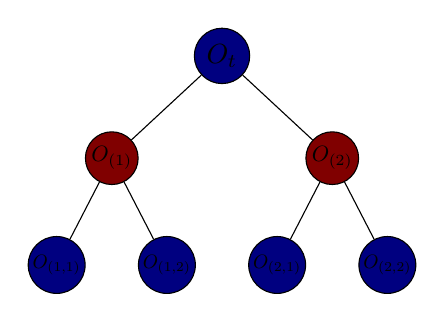
\begin{tikzpicture}
        \node[latent, fill=Blue, xshift=-0.5cm] (St) {$O_t$}; 
        \node[latent, fill=Red, below=of St, scale=0.8, yshift=0.5cm, xshift=-1.75cm] (S1) {$O_{(1)}$};
        \node[latent, fill=Red, below=of St, scale=0.8, yshift=0.5cm, xshift=1.75cm] (S2) {$O_{(2)}$};
        \node[latent, fill=Blue, below=of S2, scale=0.7, yshift=0.5cm, xshift=-1cm] (S21) {$O_{(2,1)}$};
        \node[latent, fill=Blue, below=of S2, scale=0.7, yshift=0.5cm, xshift=1cm] (S22) {$O_{(2,2)}$};
        \node[latent, fill=Blue, below=of S1, scale=0.7, yshift=0.5cm, xshift=-1cm] (S11) {$O_{(1,1)}$};
        \node[latent, fill=Blue, below=of S1, scale=0.7, yshift=0.5cm, xshift=1cm] (S12) {$O_{(1,2)}$};
        
        % edges (past and present)
        \draw[black] (St) -- (S1);
        \draw[black] (St) -- (S2);
        \draw[black] (S2) -- (S21);
        \draw[black] (S2) -- (S22);
        \draw[black] (S1) -- (S11);
        \draw[black] (S1) -- (S12);
    \end{tikzpicture}
 	\end{center}
\vspace{-0.25cm}
    \caption{
This figure illustrates a two players zero-sum game where observations are represented by nodes and actions by edges. The first player acts on blue nodes while the second player acts on red nodes.}
    \label{fig:min_max_tree}
\end{figure}
}

The MinMax algorithm provides a way of finding the optimal actions for each player. To do so, it run through the tree recursively and computes the value of each nodes. The value of leaf nodes is given by the fitness function. The red-node's value is the minimum value of its children, i.e., the opponent always try to minimise the payoff of the agent. And similarly the blue-node's value is the maximum value of its children, i.e., the agent always try to maximise its payoff. Finally, when all nodes' value have been evaluated the optimal actions are the one leading to leaf nodes whose values are the same as the root node. Figure \ref{fig:min_max_recursion} illustrates the recursive computation of the nodes' value.

{
\colorlet{Red}{red!20!white}
\colorlet{Blue}{blue!20!white}
\renewcommand\fbox{\fcolorbox{white}{white}}
\begin{figure}[H]
	\begin{center}
	\begin{tikzpicture}
	% upper-left
   \draw (-4,0) node {
	\begin{tikzpicture}
        % red and blue nodes
        \node[latent, fill=Blue, xshift=-0.5cm] (St) {$ $}; 
        \node[latent, fill=Red, below=of St, yshift=0.5cm, xshift=-1.75cm] (S1) {$ $};
        \node[latent, fill=Red, below=of St, yshift=0.5cm, xshift=1.75cm] (S2) {$ $};
        \node[latent, fill=Blue, below=of S2, yshift=0.5cm, xshift=-1cm] (S21) {$ $};
        \node[latent, fill=Blue, below=of S2, yshift=0.5cm, xshift=1cm] (S22) {$ $};
        \node[latent, fill=Blue, below=of S1, yshift=0.5cm, xshift=-1cm] (S11) {$5$};
        \node[latent, fill=Blue, below=of S1, yshift=0.5cm, xshift=1cm] (S12) {$ $};
        
        % edges
        \draw [->,very thick] (St) to [out=180,in=70] (S1);
        \draw [->,very thick] (S1) to [out=180,in=80] (S11);
        \draw[black] (St) -- (S1);
        \draw[black] (St) -- (S2);
        \draw[black] (S2) -- (S21);
        \draw[black] (S2) -- (S22);
        \draw[black] (S1) -- (S11);
        \draw[black] (S1) -- (S12);
   \end{tikzpicture}
   };
   
	% upper-right
   \draw (4,0) node {
	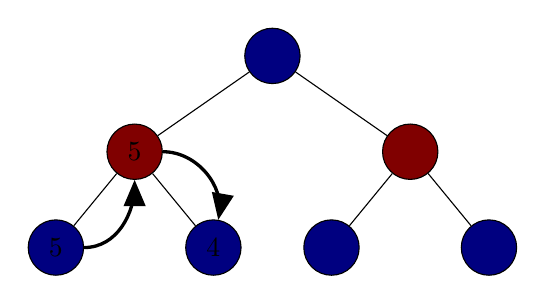
\begin{tikzpicture}
        % red and blue nodes
        \node[latent, fill=Blue, xshift=-0.5cm] (StG1) {$ $}; 
        \node[latent, fill=Red, below=of StG1, yshift=0.5cm, xshift=-1.75cm] (S1G1) {$5$};
        \node[latent, fill=Red, below=of StG1, yshift=0.5cm, xshift=1.75cm] (S2G1) {$ $};
        \node[latent, fill=Blue, below=of S2G1, yshift=0.5cm, xshift=-1cm] (S21G1) {$ $};
        \node[latent, fill=Blue, below=of S2G1, yshift=0.5cm, xshift=1cm] (S22G1) {$ $};
        \node[latent, fill=Blue, below=of S1G1, yshift=0.5cm, xshift=-1cm] (S11G1) {$5$};
        \node[latent, fill=Blue, below=of S1G1, yshift=0.5cm, xshift=1cm] (S12G1) {$4$};
        
        % edges
        \draw [->,very thick] (S11G1) to [out=0,in=270] (S1G1);
        \draw [->,very thick] (S1G1) to [out=0,in=80] (S12G1);
        \draw[black] (StG1) -- (S1G1);
        \draw[black] (StG1) -- (S2G1);
        \draw[black] (S2G1) -- (S21G1);
        \draw[black] (S2G1) -- (S22G1);
        \draw[black] (S1G1) -- (S11G1);
        \draw[black] (S1G1) -- (S12G1);
   \end{tikzpicture}
   };
   
	% middle-right
   \draw (4,-4) node {
	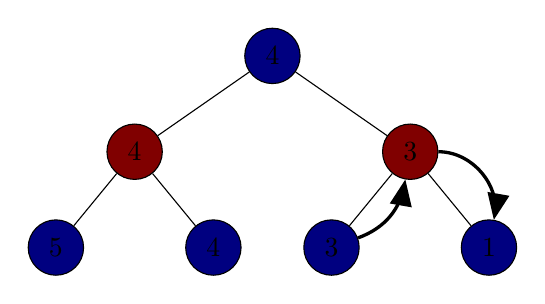
\begin{tikzpicture}
        % red and blue nodes
        \node[latent, fill=Blue, xshift=-0.5cm] (St) {$4$}; 
        \node[latent, fill=Red, below=of St, yshift=0.5cm, xshift=-1.75cm] (S1) {$4$};
        \node[latent, fill=Red, below=of St, yshift=0.5cm, xshift=1.75cm] (S2) {$3$};
        \node[latent, fill=Blue, below=of S2, yshift=0.5cm, xshift=-1cm] (S21) {$3$};
        \node[latent, fill=Blue, below=of S2, yshift=0.5cm, xshift=1cm] (S22) {$1$};
        \node[latent, fill=Blue, below=of S1, yshift=0.5cm, xshift=-1cm] (S11) {$5$};
        \node[latent, fill=Blue, below=of S1, yshift=0.5cm, xshift=1cm] (S12) {$4$};
        
        % edges
        \draw [->,very thick] (S21) to [out=20,in=260] (S2);
        \draw [->,very thick] (S2) to [out=0,in=80] (S22);
        \draw[black] (St) -- (S1);
        \draw[black] (St) -- (S2);
        \draw[black] (S2) -- (S21);
        \draw[black] (S2) -- (S22);
        \draw[black] (S1) -- (S11);
        \draw[black] (S1) -- (S12);
   \end{tikzpicture}
   };

	% middle-left
   \draw (-4,-4) node {
	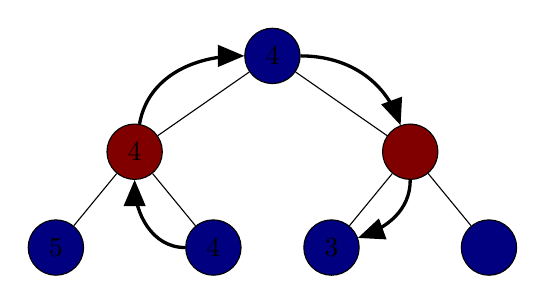
\begin{tikzpicture}
        % red and blue nodes
        \node[latent, fill=Blue, xshift=-0.5cm] (St) {$4$}; 
        \node[latent, fill=Red, below=of St, yshift=0.5cm, xshift=-1.75cm] (S1) {$4$};
        \node[latent, fill=Red, below=of St, yshift=0.5cm, xshift=1.75cm] (S2) {$ $};
        \node[latent, fill=Blue, below=of S2, yshift=0.5cm, xshift=-1cm] (S21) {$3$};
        \node[latent, fill=Blue, below=of S2, yshift=0.5cm, xshift=1cm] (S22) {$ $};
        \node[latent, fill=Blue, below=of S1, yshift=0.5cm, xshift=-1cm] (S11) {$5$};
        \node[latent, fill=Blue, below=of S1, yshift=0.5cm, xshift=1cm] (S12) {$4$};
        
        % edges
        \draw [->,very thick] (S12) to [out=180,in=270] (S1);
        \draw [->,very thick] (S1) to [out=80,in=180] (St);
        \draw [->,very thick] (St) to [out=0,in=110] (S2);
        \draw [->,very thick] (S2) to [out=270,in=20] (S21);
        \draw[black] (St) -- (S1);
        \draw[black] (St) -- (S2);
        \draw[black] (S2) -- (S21);
        \draw[black] (S2) -- (S22);
        \draw[black] (S1) -- (S11);
        \draw[black] (S1) -- (S12);
   \end{tikzpicture}
   };

	% bottom-center
   \draw (0,-8) node {
	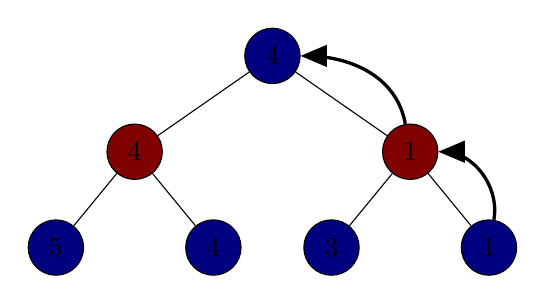
\begin{tikzpicture}
        % red and blue nodes
        \node[latent, fill=Blue, xshift=-0.5cm] (St) {$4$}; 
        \node[latent, fill=Red, below=of St, yshift=0.5cm, xshift=-1.75cm] (S1) {$4$};
        \node[latent, fill=Red, below=of St, yshift=0.5cm, xshift=1.75cm] (S2) {$1$};
        \node[latent, fill=Blue, below=of S2, yshift=0.5cm, xshift=-1cm] (S21) {$3$};
        \node[latent, fill=Blue, below=of S2, yshift=0.5cm, xshift=1cm] (S22) {$1$};
        \node[latent, fill=Blue, below=of S1, yshift=0.5cm, xshift=-1cm] (S11) {$5$};
        \node[latent, fill=Blue, below=of S1, yshift=0.5cm, xshift=1cm] (S12) {$4$};
        
        % edges
        \draw [->,very thick] (S22) to [out=80,in=0] (S2);
        \draw [->,very thick] (S2) to [out=100,in=0] (St);
        \draw[black] (St) -- (S1);
        \draw[black] (St) -- (S2);
        \draw[black] (S2) -- (S21);
        \draw[black] (S2) -- (S22);
        \draw[black] (S1) -- (S11);
        \draw[black] (S1) -- (S12);
   \end{tikzpicture}
   };
   
   \end{tikzpicture}
 	\end{center}
\vspace{-0.25cm}
    \caption{
This figure illustrates the recursive computation of the nodes' value. This figure must be read from left to right and from top to bottom. Each time the recursion reach a leaf node, the fitness function is used to evaluate its value. Each time a value is back-propagated toward a red node, only the smallest value is conserved. And finally, each time a value is back-propagated toward a blue node, only the largest value is conserved.}
    \label{fig:min_max_recursion}
\end{figure}
}

\subsection*{Pseudo code}

\begin{minted}[escapeinside=||,mathescape=true]{python}
function minimax(node)
    # Each leaf node returns its value
    if node.isLeafNode()
        return fitness(node)
    # Each node where the agent must play 
    # returns the maximal value of its children
    if node.isAgentTurn()
        value = |$-\infty$|
        for child in node.children()
            value = max(value, minimax(child))
        return value
    # Each node where the opponent must play
    # returns the minimal value of its children
    value = |$+\infty$|
    for child in node.children()
        value = min(value, minimax(child))
    return value
\end{minted}

\section{MinMax with alpha-beta pruning}

\subsection*{Notations}

This section re-uses the notations of Section \ref{sec:minmax}. Also for each node where the agent has to play (i.e., blue nodes), let $\alpha$ be the maximum value of the node's children already explored, i.e., the maximal payoff that the agent can safely secure from this blue node. Similarly, for each node where the opponent has to play (i.e., red nodes), let $\beta$ be the minimum value of the node's children already explored, i.e., the lowest payoff that the opponent can safely secure from this red node.

\subsection*{Algorithm description}

The MinMax algorithm with alpha-beta pruning leads to the same result as the MinMax algorithm, but cut off branches that don't need to be explored making the algorithm faster. Put simply, each time a value is back-propagate toward a red node, the algorithm updates the red-node's $\beta$ such as it remains equal to the minimal value of the red-node's children. Furthermore, if during the update $\beta$ drops below the value of $\alpha$ of the red-node's parent then the remaining red-node's children are cut off and will not be evaluated. Similarly, each time a value is back-propagate toward a blue node, the algorithm updates the blue-node's $\alpha$ such as it remains equal to the maximal value of the blue-node's children. Furthermore, if during the update $\alpha$ becomes bigger than the value of $\beta$ of the blue-node's parent then the remaining blue-node's children are cut off and will not be evaluated. Figure \ref{fig:alpha_beta_pruning} illustrates the MinMax algorithm with alpha-beta pruning.

{
\colorlet{DarkRed}{red!80!black}
\colorlet{LightGray}{lightgray!30!white}
\colorlet{Red}{red!20!white}
\colorlet{Blue}{blue!20!white}
\colorlet{Green}{green!80!black}
\colorlet{Orange}{orange!80!black}
\renewcommand\fbox{\fcolorbox{white}{white}}
\begin{figure}[H]
	\begin{center}
	\begin{tikzpicture}[square/.style={regular polygon,regular polygon sides=4}]
	% upper-left
   \draw (-4,0) node {
	\begin{tikzpicture}
        % red and blue nodes
        \node[latent, fill=Blue, xshift=-0.5cm] (St) {$ $}; 
        \node[latent, fill=Red, below=of St, yshift=0.5cm, xshift=-1.75cm] (S1) {$ $};
        \node[latent, fill=Red, below=of St, yshift=0.5cm, xshift=1.75cm] (S2) {$ $};
        \node[latent, fill=Blue, below=of S2, yshift=0.5cm, xshift=-1cm] (S21) {$ $};
        \node[latent, fill=Blue, below=of S2, yshift=0.5cm, xshift=1cm] (S22) {$ $};
        \node[latent, fill=Blue, below=of S1, yshift=0.5cm, xshift=-1cm] (S11) {$5$};
        \node[latent, fill=Blue, below=of S1, yshift=0.5cm, xshift=1cm] (S12) {$ $};
        
        % edges
        \draw [->,very thick] (St) to [out=180,in=70] (S1);
        \draw [->,very thick] (S1) to [out=180,in=80] (S11);
        \draw[black] (St) -- (S1);
        \draw[black] (St) -- (S2);
        \draw[black] (S2) -- (S21);
        \draw[black] (S2) -- (S22);
        \draw[black] (S1) -- (S11);
        \draw[black] (S1) -- (S12);
        
        % green and orange nodes
        \node[latent, square, draw=Green, above= of St, yshift=-0.5cm, scale=0.5] (alphaSt) {$\bm{-\infty}$}; 
        \draw[Green] (St) -- (alphaSt);

        \node[latent, square, draw=Orange, above= of S1, yshift=-0.5cm, scale=0.5] (alphaS1) {$\bm{-\infty}$}; 
        \draw[Orange] (S1) -- (alphaS1);

        \node[latent, square, draw=Orange, above= of S2, yshift=-0.5cm, scale=0.5] (alphaS2) {$\bm{-\infty}$}; 
        \draw[Orange] (S2) -- (alphaS2);
   \end{tikzpicture}
   };
   
	% upper-right
   \draw (4,0) node {
	\begin{tikzpicture}
        % red and blue nodes
        \node[latent, fill=Blue, xshift=-0.5cm] (StG1) {$ $}; 
        \node[latent, fill=Red, below=of StG1, yshift=0.5cm, xshift=-1.75cm] (S1G1) {$5$};
        \node[latent, fill=Red, below=of StG1, yshift=0.5cm, xshift=1.75cm] (S2G1) {$ $};
        \node[latent, fill=Blue, below=of S2G1, yshift=0.5cm, xshift=-1cm] (S21G1) {$ $};
        \node[latent, fill=Blue, below=of S2G1, yshift=0.5cm, xshift=1cm] (S22G1) {$ $};
        \node[latent, fill=Blue, below=of S1G1, yshift=0.5cm, xshift=-1cm] (S11G1) {$5$};
        \node[latent, fill=Blue, below=of S1G1, yshift=0.5cm, xshift=1cm] (S12G1) {$4$};
        
        % edges
        \draw [->,very thick] (S11G1) to [out=0,in=270] (S1G1);
        \draw [->,very thick] (S1G1) to [out=0,in=80] (S12G1);
        \draw[black] (StG1) -- (S1G1);
        \draw[black] (StG1) -- (S2G1);
        \draw[black] (S2G1) -- (S21G1);
        \draw[black] (S2G1) -- (S22G1);
        \draw[black] (S1G1) -- (S11G1);
        \draw[black] (S1G1) -- (S12G1);   
             
        % green and orange nodes
        \node[latent, square, draw=Green, above= of St, yshift=-0.5cm, scale=0.5] (alphaSt) {$\bm{-\infty}$}; 
        \draw[Green] (St) -- (alphaSt);

        \node[latent, square, draw=Orange, above= of S1, yshift=-0.5cm] (alphaS1) {$5$}; 
        \draw[Orange] (S1) -- (alphaS1);

        \node[latent, square, draw=Orange, above= of S2, yshift=-0.5cm, scale=0.5] (alphaS2) {$\bm{-\infty}$}; 
        \draw[Orange] (S2) -- (alphaS2);
   \end{tikzpicture}
   };
   
	% lower-right
   \draw (4,-5) node {
	\begin{tikzpicture}
        % red and blue nodes
        \node[latent, fill=Blue, xshift=-0.5cm] (St) {$4$}; 
        \node[latent, fill=Red, below=of St, yshift=0.5cm, xshift=-1.75cm] (S1) {$4$};
        \node[latent, fill=Red, below=of St, yshift=0.5cm, xshift=1.75cm] (S2) {$3$};
        \node[latent, fill=Blue, below=of S2, yshift=0.5cm, xshift=-1cm] (S21) {$3$};
        \node[latent, fill=LightGray, draw=lightgray, below=of S2, yshift=0.5cm, xshift=1cm] (S22) {$ $};
        \node[latent, fill=Blue, below=of S1, yshift=0.5cm, xshift=-1cm] (S11) {$5$};
        \node[latent, fill=Blue, below=of S1, yshift=0.5cm, xshift=1cm] (S12) {$4$};
        
        % edges
        \draw [->,very thick] (S21) to [out=20,in=260] (S2);
        \draw [->,very thick] (S2) to [out=100,in=0] (St);
        \draw[black] (St) -- (S1);
        \draw[black] (St) -- (S2);
        \draw[black] (S2) -- (S21);
        \draw[lightgray] (S2) -- (S22);
        \draw[black] (S1) -- (S11);
        \draw[black] (S1) -- (S12);
        \draw [DarkRed, very thick] (1.5,-2.0) -- (2.0,-1.6);
                
        % green and orange nodes
        \node[latent, square, draw=Green, above= of St, yshift=-0.5cm] (alphaSt) {$4$}; 
        \draw[Green] (St) -- (alphaSt);

        \node[latent, square, draw=Orange, above= of S1, yshift=-0.5cm] (alphaS1) {$4$}; 
        \draw[Orange] (S1) -- (alphaS1);

        \node[latent, square, draw=Orange, above= of S2, yshift=-0.5cm] (alphaS2) {$3$}; 
        \draw[Orange] (S2) -- (alphaS2);
   \end{tikzpicture}
   };

	% lower-left
   \draw (-4,-5) node {
	\begin{tikzpicture}
        % red and blue nodes
        \node[latent, fill=Blue, xshift=-0.5cm] (St) {$4$}; 
        \node[latent, fill=Red, below=of St, yshift=0.5cm, xshift=-1.75cm] (S1) {$4$};
        \node[latent, fill=Red, below=of St, yshift=0.5cm, xshift=1.75cm] (S2) {$ $};
        \node[latent, fill=Blue, below=of S2, yshift=0.5cm, xshift=-1cm] (S21) {$3$};
        \node[latent, fill=Blue, below=of S2, yshift=0.5cm, xshift=1cm] (S22) {$ $};
        \node[latent, fill=Blue, below=of S1, yshift=0.5cm, xshift=-1cm] (S11) {$5$};
        \node[latent, fill=Blue, below=of S1, yshift=0.5cm, xshift=1cm] (S12) {$4$};
        
        % edges
        \draw [->,very thick] (S12) to [out=180,in=270] (S1);
        \draw [->,very thick] (S1) to [out=80,in=180] (St);
        \draw [->,very thick] (St) to [out=0,in=110] (S2);
        \draw [->,very thick] (S2) to [out=270,in=20] (S21);
        \draw[black] (St) -- (S1);
        \draw[black] (St) -- (S2);
        \draw[black] (S2) -- (S21);
        \draw[black] (S2) -- (S22);
        \draw[black] (S1) -- (S11);
        \draw[black] (S1) -- (S12);
                
        % green and orange nodes
        \node[latent, square, draw=Green, above= of St, yshift=-0.5cm] (alphaSt) {$4$}; 
        \draw[Green] (St) -- (alphaSt);

        \node[latent, square, draw=Orange, above= of S1, yshift=-0.5cm] (alphaS1) {$4$}; 
        \draw[Orange] (S1) -- (alphaS1);

        \node[latent, square, draw=Orange, above= of S2, yshift=-0.5cm, scale=0.5] (alphaS2) {$\bm{-\infty}$}; 
        \draw[Orange] (S2) -- (alphaS2);
   \end{tikzpicture}
   };
   
   \end{tikzpicture}
 	\end{center}
\vspace{-0.25cm}
    \caption{
This figure illustrates the recursive computation of the nodes' value where green and orange nodes represent value of $\alpha$ and $\beta$, respectively. Each time a value is back-propagated toward a red node, the corresponding value of $\beta$ is updated. Each time a value is back-propagated toward a blue node, the corresponding value of $\alpha$ is updated. Finally, when the $\beta$ value of a red node drops below the $\alpha$ value of the red-node's parent the remaining child branches are cut off, c.f. lower-right corner.}
    \label{fig:alpha_beta_pruning}
\end{figure}
}

\subsection*{Pseudo code}

\begin{minted}[escapeinside=||,mathescape=true]{python}
function alphabeta(node, |$\alpha$|, |$\beta$|)
    # Each leaf node returns its value
    if node.isLeafNode()
        return fitness(node)
    # Each node where the agent must play returns the maximal value 
    # of its children. The evaluation of the child nodes is stopped 
    # when the value of a child (i.e., $\alpha$) is superior to the 
    # minimal value already found by the node's parent (i.e., $\beta$).
    # Indeed, the opponent will not select this branch because it 
    # has already found a branch with a lower payoff.
    if node.isAgentTurn()
        value = |$-\infty$|
        for child in node.children()
            value = max(value, alphabeta(child, |$\alpha$|, |$\beta$|))
            |$\alpha$| = max(|$\alpha$|, value)
            if |$\alpha \geq \beta$|
                break # $\beta$ cutoff
        return value
    # Each node where the opponent must play returns the minimal 
    # value of its children. The evaluation of the child nodes is 
    # stopped when the value of a child (i.e., $\beta$) is inferior to 
    # the maximal value already found by the node's parent (i.e., $\alpha$).
    # Indeed, the agent will not select this branch because it 
    # has already found a branch with a higher payoff.
    value = |$+\infty$|
    for child in node.children()
        value = min(value, alphabeta(child, |$\alpha$|, |$\beta$|))
        |$\beta$| = min(|$\beta$|, value)
        if |$\beta \leq \alpha$|
            break # $\alpha$ cutoff
    return value
\end{minted}

%----------------------------------------------------------------------------------------
%	CHAPTER 4
%----------------------------------------------------------------------------------------

\chapterimage{Chapter4Image.png}
\chapter{Probabilistic Graphical Model}

\section{Bayesian Network}

\section{Normal Factor Graph}

\cite{FFG}

\section{Factor Graph}

\section{Markov Random Field}

\vskip 0.2in
\bibliographystyle{apalike}
\bibliography{references}

% Chapter template:
%\chapterimage{head2.png}
%\chapter{Convex Sets}
%\section{Convexity}
%\subsection{Cone}

% Remark template:
%\begin{remark}
%\begin{itemize}
%\item $f$ is 2nd-differentiable, $f$ ix \cvx $\iff$ $\nabla^2f(x) \rangle  0$.
%\item $f$ is strongly \cvx $\iff$ $\nabla^2f(x) \rangle  \mu I$ $\iff$ $x \ge \mu$
%\end{itemize}
%\end{remark}

% Definition template:
% \begin{definition}[Epigraph]
% For $f: \R^n \rightarrow \bar{R}$, its epigraph $epi(f) \in \R^{n+1} is the set epi(f) \{ (x,\alpha) | f(x) \in \alpha \}$
% \end{definition}

% Example template:
%\begin{example}[L2-norm]
%$\|x \|_p = \sup \{ \langle x, u \rangle, u \in B_q \}$ where $\frac{1}{p} + \frac{1}{q} = 1$. $B_q = \{ \|x \|_q \le 1\}$.\\
%\end{example}

% Fact template:
%\begin{fact}[Epigraph of a support function]
%$epi \space \sigma_C = \{ (x,t) | \sigma_C(x) \le t\}$.
%Suppose $(x,t) \in epi \space \sigma_C$. Take any  $\alpha > 0$. $\alpha(x,t) = (\alpha x, \alpha t)$.\\
%$\alpha \sigma_C(x) = \alpha \sigma_C(x) \le \alpha t$. $\alpha(x,c) \in epi 
%\sigma_C$\\
%\end{fact}

% Proof template:
%\begin{proof}
%$\Rightarrow$ take $x,y \in dom \space f$, $(x,f(x)) \in epi \space f$,$(y,f(y)) \in epi \space f$.
%\end{proof}

% Theorem template:
%\begin{theorem}
%$f : \R^n \to \bar{\R}$ is \cvx  $\iff$ $\forall x,y \in \R^n, \alpha \in (0,1), f(ax + (1-a)x) \le af(x) + (1-a)f(x)$.
%\end{theorem}

\end{document}